\documentclass[11pt,a4paper]{article}
\usepackage[utf8]{inputenc}
\usepackage[T1]{fontenc}
\usepackage{graphicx}
\usepackage{hyperref}
\usepackage{xcolor}
\usepackage{geometry}
\usepackage{enumitem}
\usepackage{tabularx}
\usepackage{booktabs}
\usepackage{tikz}
\usepackage{float}
\usepackage{fancyhdr}
\usepackage{amssymb} % For diamond symbol

% Set page margins
\geometry{a4paper, margin=1in}

% Define colors
\definecolor{headingblue}{RGB}{0, 51, 102}
\definecolor{lightblue}{RGB}{179, 209, 255}

% Header and footer setup
\pagestyle{fancy}
\fancyhf{}
\renewcommand{\headrulewidth}{1pt}
\renewcommand{\footrulewidth}{0.5pt}
\fancyhead[L]{TIES454 - Agentic Technologies for Developers}
\fancyhead[R]{Team G.O.A.T}
\fancyfoot[C]{Page \thepage}

% Title setup
\title{
    {\LARGE\textbf{Research Assistant Multi-Agent System}}\\
    \vspace{0.5cm}
    {\large\textbf{Design using GAIA Methodology}}\\
    \vspace{0.5cm}
}
\author{Abdelaziz Ibrahim \and Besher Alkurdi \and Bishwash Khanal}
\date{\today}

\begin{document}

\maketitle
\thispagestyle{fancy}

\section*{Problem Domain}
\subsection*{Background}
Research literature review is crucial but presents significant challenges:
\begin{itemize}
    \item Manual literature review is time-consuming and prone to overlooking relevant work
    \item PhD students need to quickly understand the state-of-the-art in new fields
    \item Research teams need to identify contradictory findings across multiple studies
    \item Processing the sheer volume of available research papers is overwhelming
\end{itemize}

\subsection*{Importance}
A comprehensive literature review is essential when:
\begin{itemize}
    \item Writing academic papers and theses
    \item Starting to research already explored ideas
    \item Understanding a topic deeply to find research gaps
    \item Avoiding duplication of efforts in academic research
\end{itemize}

\subsection*{Challenges}
\begin{itemize}
    \item \textbf{Information Overload:} The sheer volume of available research papers is overwhelming
    \item \textbf{Quality Assessment:} Determining the relevance and reliability of sources is difficult
    \item \textbf{Synthesis Complexity:} Connecting findings across diverse studies requires significant expertise
    \item \textbf{Time Constraints:} Thoroughly processing and extracting meaningful insights from each source is time-consuming
\end{itemize}

\section{Multi-Agent System Design}

\subsection{Analysis Phase}

\subsubsection{Environmental Model}
The environmental model represents the abstract and computational environment where our MAS will operate. The diagram below shows key resources that agents will interact with:

\begin{figure}[H]
    \centering
    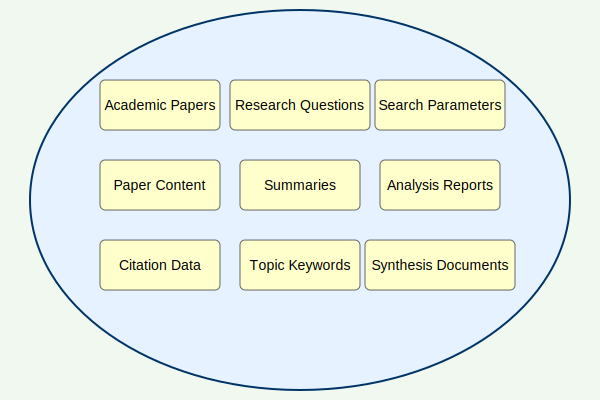
\includegraphics[width=0.8\textwidth]{images/environmental-model.png}
    \caption{Environmental Model for Research Assistant MAS}
    \label{fig:env-model}
\end{figure}

\subsubsection{Preliminary Role and Interaction Models}

We have identified two key scenarios that our multi-agent system will address:

\paragraph{Scenario 1: Comprehensive Literature Collection}
\begin{itemize}
    \item \textbf{Challenge:} Researchers struggle to find all relevant papers across multiple databases and repositories.
    \item \textbf{Solution:} The Search Agent automatically queries multiple academic sources (Google Scholar, arXiv, PubMed), collecting comprehensive results beyond what a human could manually gather.
\end{itemize}

\begin{figure}[H]
    \centering
    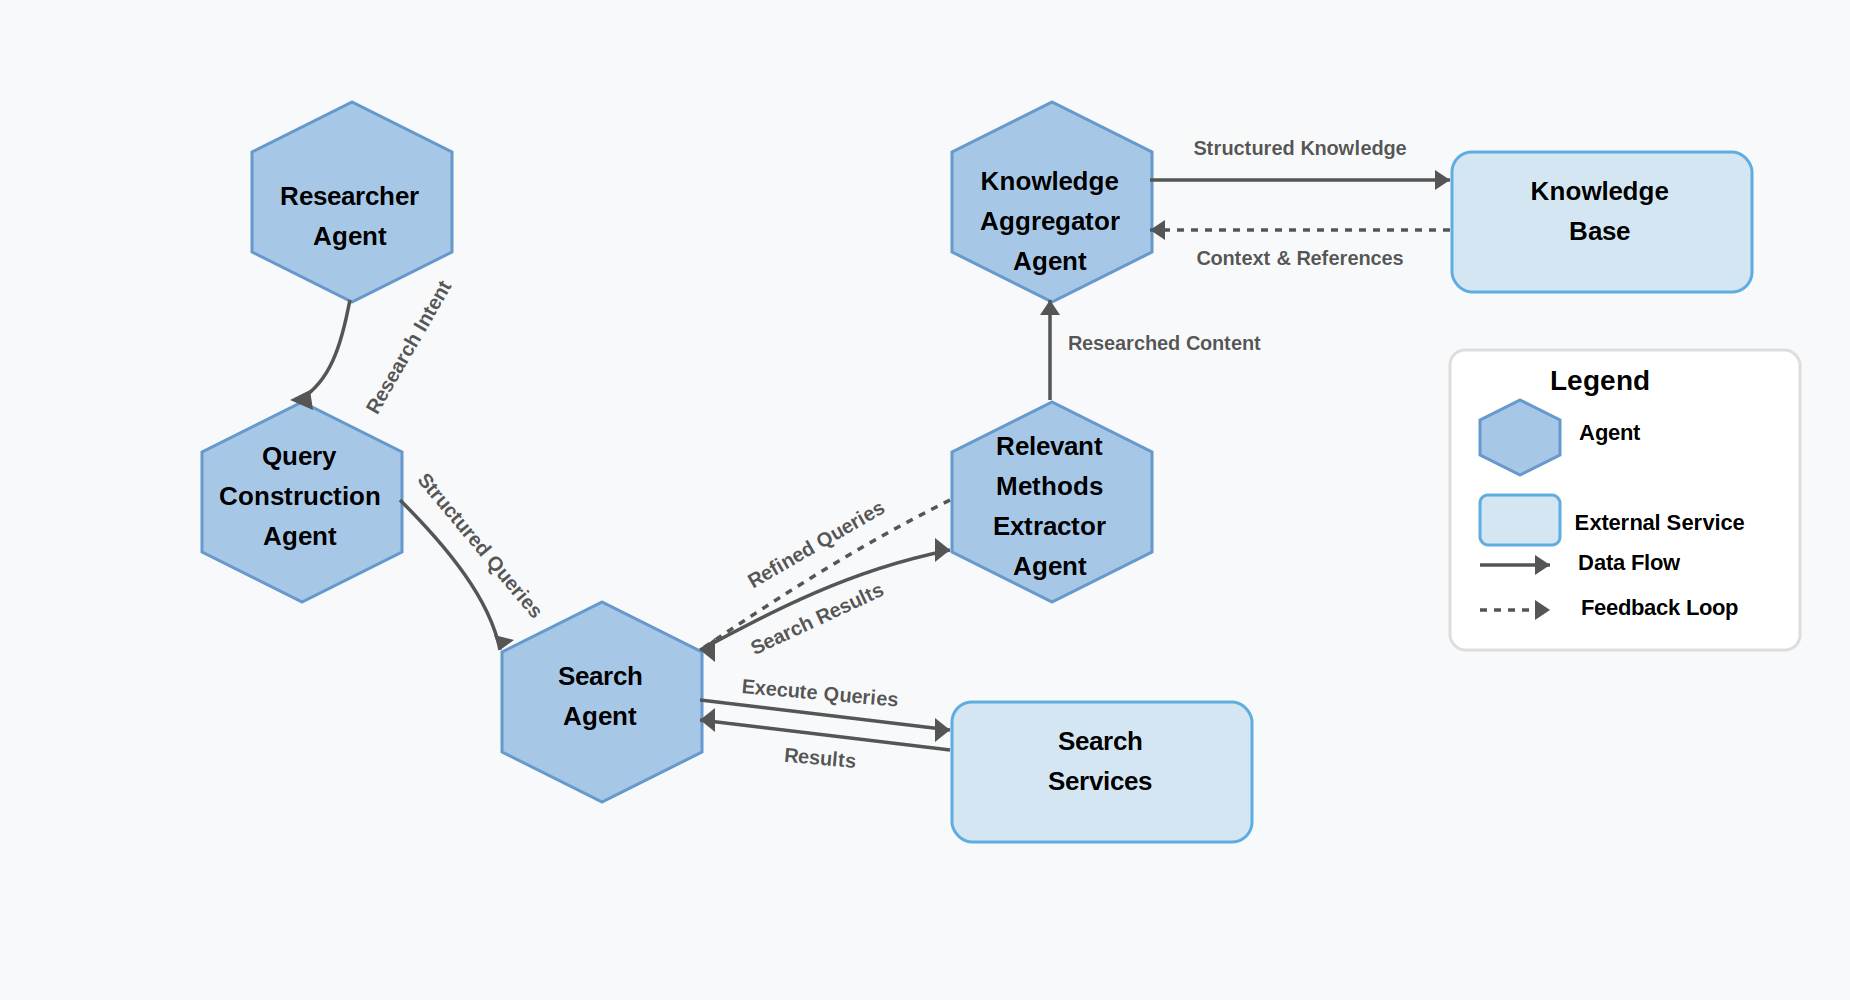
\includegraphics[width=0.8\textwidth]{images/preliminary-roles-scenario1.png}
    \caption{Preliminary Roles and Interactions for Scenario 1}
    \label{fig:scenario1}
\end{figure}

\paragraph{Scenario 2: Content Analysis and Synthesis}
\begin{itemize}
    \item \textbf{Challenge:} Extracting key findings from dozens of papers is time-consuming and prone to oversight.
    \item \textbf{Solution:} The Analysis Agent reads papers, extracting methodologies and findings, while the Synthesis Agent connects related concepts across papers, identifying research gaps.
\end{itemize}

\begin{figure}[H]
    \centering
    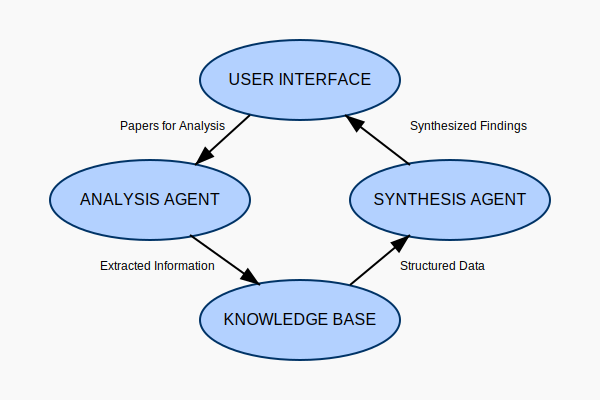
\includegraphics[width=0.8\textwidth]{images/preliminary-roles-scenario2.png}
    \caption{Preliminary Roles and Interactions for Scenario 2}
    \label{fig:scenario2}
\end{figure}

% \subsubsection{Organizational Rules}
% The following organizational rules govern the interactions between agents in our system:

% \begin{enumerate}
%     \item Each research query must be processed by at least one Search Agent: \\
%     $\forall q.card(SEARCH\_AGENT(q)) \geq 1$
    
%     \item A Query Agent cannot evaluate its own search parameters: \\
%     $\forall q. \forall a: plays(a, QUERY\_AGENT(q)) \Rightarrow \neg plays(a, SEARCH\_EVALUATOR(q))$
    
%     \item If a paper is found, it must be analyzed: \\
%     $\forall p. participate(r, FindPaper(p)) \Rightarrow \lozenge initiate(r, AnalyzePaper(p))$
    
%     \item Every analyzed paper must be included in the knowledge base: \\
%     $\forall p. participate(r, AnalyzePaper(p)) \Rightarrow \lozenge initiate(r, StoreInKnowledgeBase(p))$
% \end{enumerate}

\subsection{Architectural Design}

\subsubsection{Role Model}
Below is a detailed role schema for the Search Agent, one of the key roles in our system:

\begin{figure}[H]
    \centering
    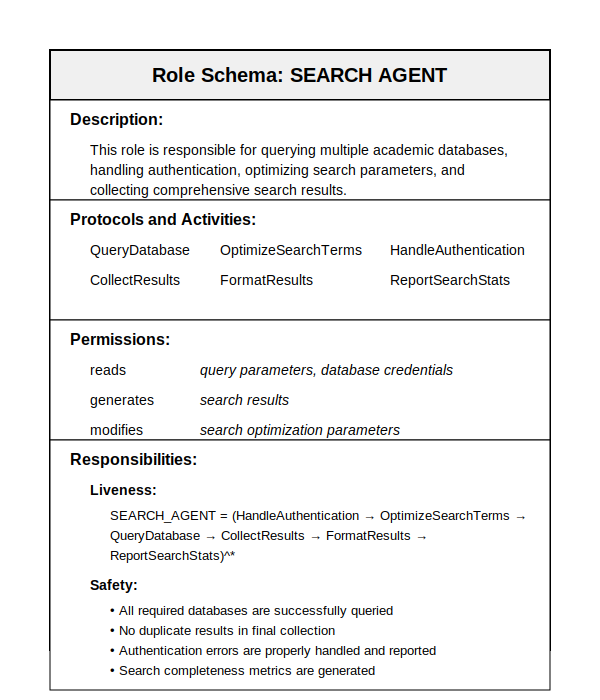
\includegraphics[width=0.8\textwidth]{images/role-model.png}
    \caption{Role Schema for Search Agent}
    \label{fig:role-model}
\end{figure}

\subsubsection{Interaction Model}
The interaction model defines the communication protocols between agents:

\begin{table}[H]
    \centering
    \begin{tabular}{|p{3cm}|p{2.5cm}|p{2.5cm}|p{3cm}|p{3cm}|}
    \hline
    \textbf{Protocol Name} & \textbf{Initiator} & \textbf{Partner} & \textbf{Inputs} & \textbf{Outputs} \\
    \hline
    FormulateQuery & User & Researcher Agent & Research question & Search parameters \\
    \hline
    QueryDatabase & Search Agent & Search Services & Search parameters & Raw results \\
    \hline
    AggregateResults & Knowledge Aggregator Agent & Relevan Methods Extractor Agent & Related Research & Knowledge Base \\
    \hline
    AnalyzePaper & Analysis Agent & Knowledge Aggregator Agent & Knowledge Base &  Methodologies and Findings report \\
    \hline
    SynthesizeFindings & Synthesis Agent & Summarization Agent & Summarized Methodologies and Findings & Synthesis Report \\
    \hline
    PresentFindings & User & Synthesis Agent & Synthesis report & Visualized findings \\
    \hline
    \end{tabular}
    \caption{Interaction Model for Research Assistant MAS}
    \label{tab:interaction-model}
\end{table}

% \subsubsection{Organizational Structure}
% The organizational structure of our MAS is as follows:

% \begin{figure}[H]
%     \centering
%     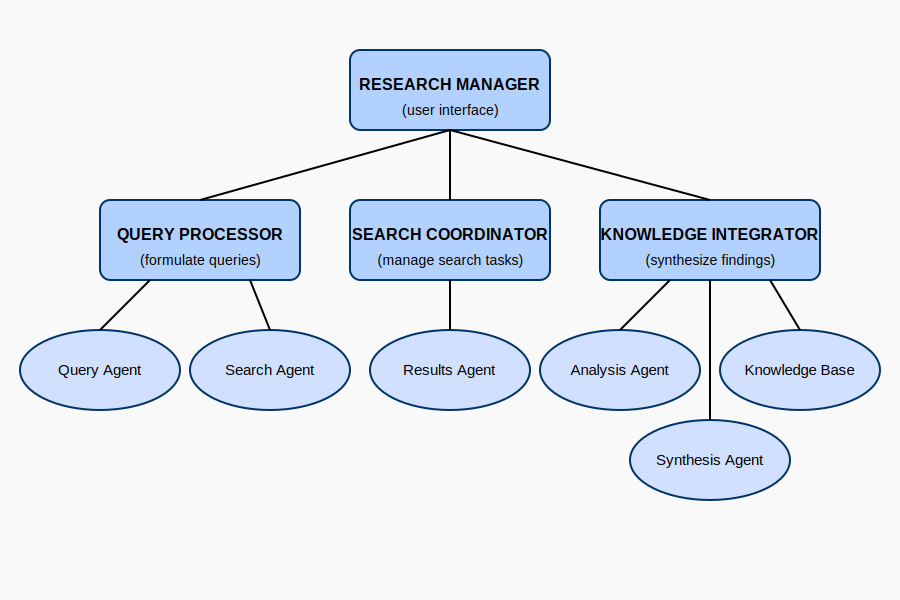
\includegraphics[width=\textwidth]{images/organizational-structure.png}
%     \caption{Organizational Structure for Research Assistant MAS}
%     \label{fig:org-structure}
% \end{figure}

\subsection{Detailed Design}

\subsubsection{Agent Model}
The agent model maps roles to specific agent types:

\begin{figure}[H]
    \centering
    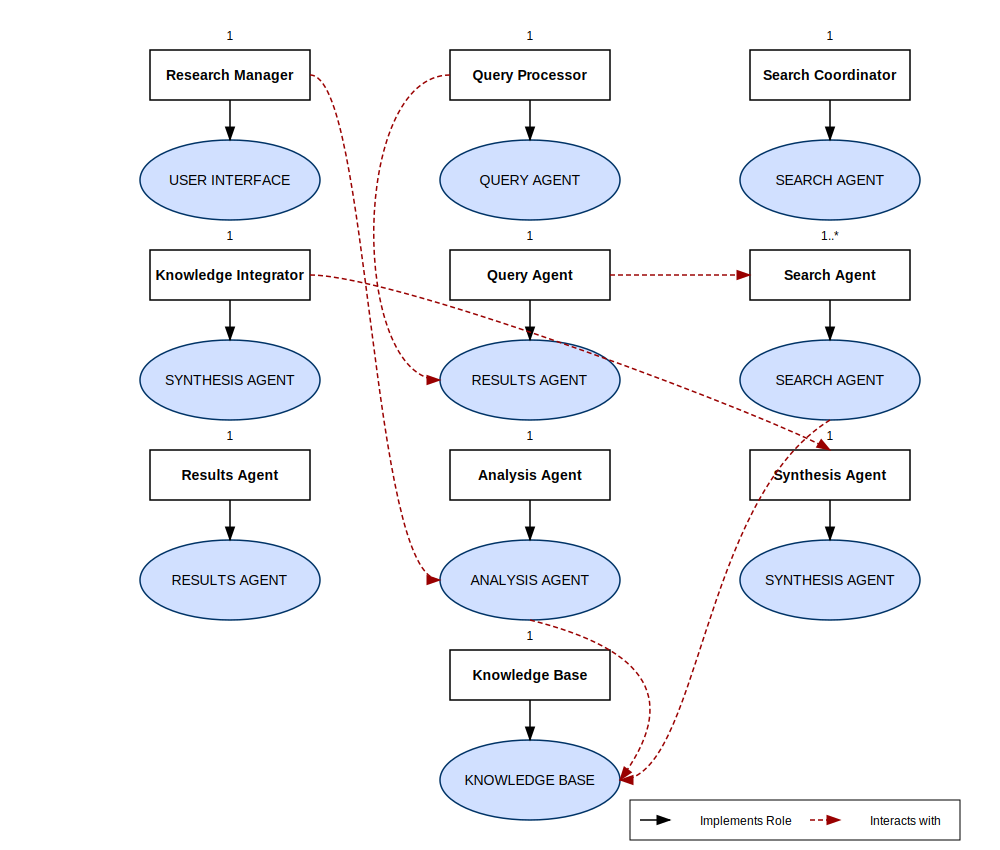
\includegraphics[width=0.7\textwidth]{images/agent-model.png}
    \caption{Agent Model for Research Assistant MAS}
    \label{fig:agent-model}
\end{figure}

\subsubsection{Service Model}
The service model defines the services offered by each agent type:

\begin{table}[H]
    \centering
    \begin{tabular}{|p{2.5cm}|p{3cm}|p{2.5cm}|p{3cm}|p{3cm}|}
    \hline
    \textbf{Service} & \textbf{Input} & \textbf{Output} & \textbf{Pre-condition} & \textbf{Post-condition} \\
    \hline
    QueryDatabase & Search parameters, credentials & Raw search results & Authentication successful & Results collected from database \\
    \hline
    OptimizeSearch & Initial parameters, research context & Optimized query & Initial parameters provided & Expanded query with synonyms \\
    \hline
    CollectResults & Raw results from multiple databases & Consolidated result set & Search operations completed & Duplicates removed \\
    \hline
    AnalyzePaper & Paper content & Structured analysis (methods, findings) & Full text available & Key information extracted \\
    \hline
    SynthesizeFindings & Multiple paper analyses & Synthesis report with trends & Multiple papers analyzed & Connections between papers identified \\
    \hline
    \end{tabular}
    \caption{Service Model for Research Assistant MAS}
    \label{tab:service-model}
\end{table}

\end{document}